\documentclass[11pt]{article}
\usepackage{textcomp,geometry,graphicx,verbatim}
\usepackage{fancyhdr}
\usepackage{amsmath,amssymb,enumerate}
\pagestyle{fancy}
\def\Name{Manohar Jois}
\def\Homework{1} % Homework number - make sure to change for every homework!
\def\Session{Spring 2015}

% Extra commands
\let\origleft\left
\let\origright\right
\renewcommand{\left}{\mathopen{}\mathclose\bgroup\origleft}
\renewcommand{\right}{\aftergroup\egroup\origright}
\newcommand{\N}{\mathbb{N}}
\newcommand{\Z}{\mathbb{Z}}
\newcommand{\R}{\mathbb{R}}
\newcommand{\Q}{\mathbb{Q}}
\newcommand{\C}{\mathbb{C}}
\newcommand{\p}[1]{\left(#1\right)}
\renewcommand{\gcd}[1]{\text{gcd}\p{#1}}
\renewcommand{\deg}[1]{\text{deg}\p{#1}}
\renewcommand{\log}[1]{\text{log}\p{#1}}
\renewcommand{\ln}[1]{\text{ln}\p{#1}}
\newcommand{\logb}[2]{\text{log}_{#1}\p{#2}}
\newcommand{\BigOh}[1]{O\p{#1}}
\newcommand{\BigOmega}[1]{\Omega\p{#1}}
\newcommand{\BigTheta}[1]{\Theta\p{#1}}
\newcommand{\asdf}{\newline\newline}

\title{CS189\ \Session\  --- Answers to Homework \Homework}
\author{\Name}
\lhead{CS189\ \Session\  Homework \Homework\ Problem \theproblemnumber,\ \Name}

\begin{document}
\maketitle
\newcounter{problemnumber}
\setcounter{problemnumber}{0}

\section*{Problem 1}
\stepcounter{problemnumber}
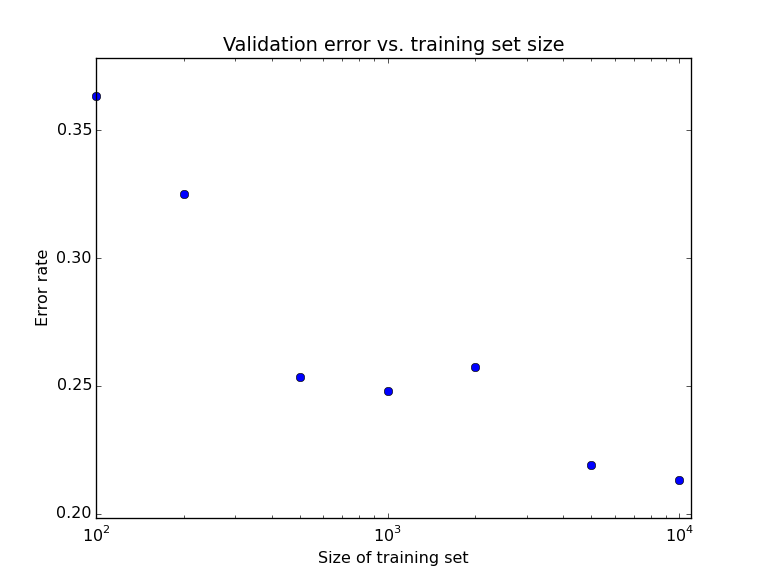
\includegraphics[scale=0.8]{images/error_rates}


\newpage
\section*{Problem 2}
\stepcounter{problemnumber}
\begin{tabular}{cc}
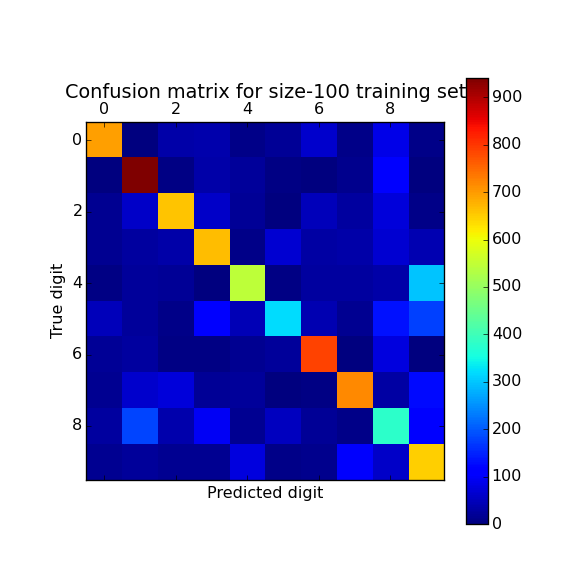
\includegraphics[scale=0.5]{images/confusion_matrix_100} & 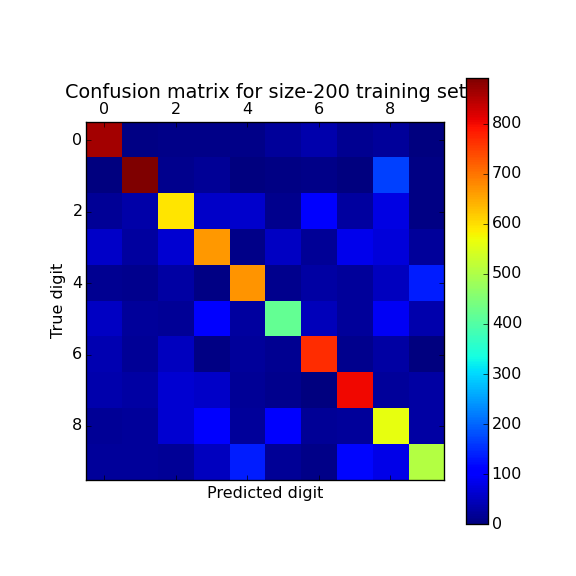
\includegraphics[scale=0.5]{images/confusion_matrix_200} \\
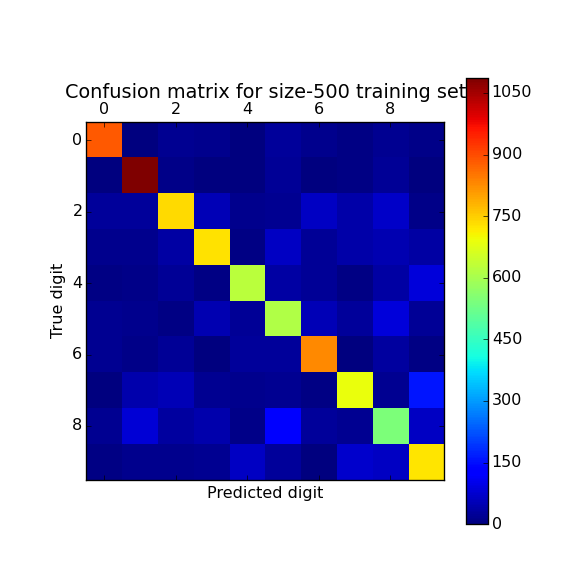
\includegraphics[scale=0.5]{images/confusion_matrix_500} & 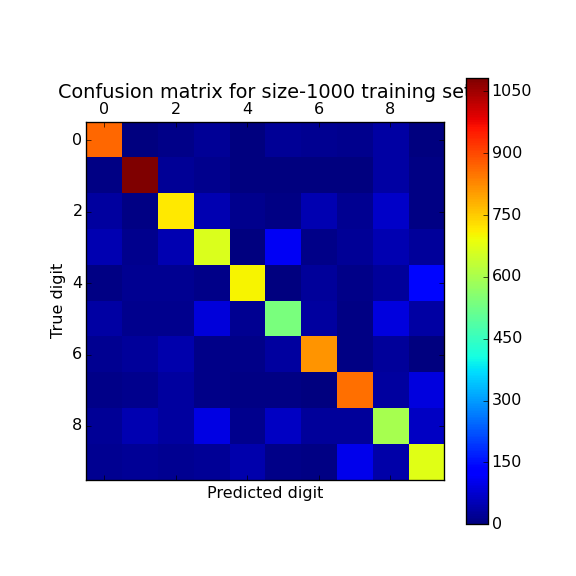
\includegraphics[scale=0.5]{images/confusion_matrix_1000}
\end{tabular}
\newpage
\begin{tabular}{cc}
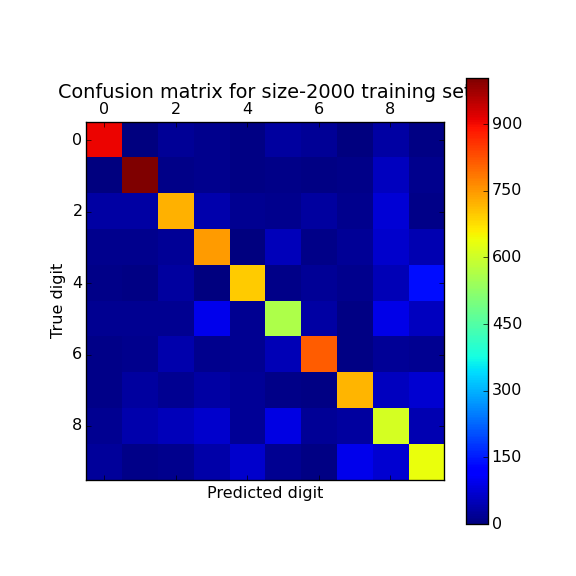
\includegraphics[scale=0.5]{images/confusion_matrix_2000} & 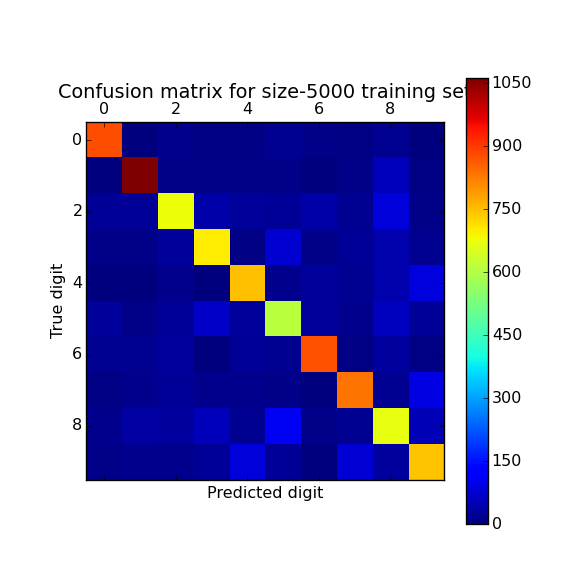
\includegraphics[scale=0.5]{images/confusion_matrix_5000} \\
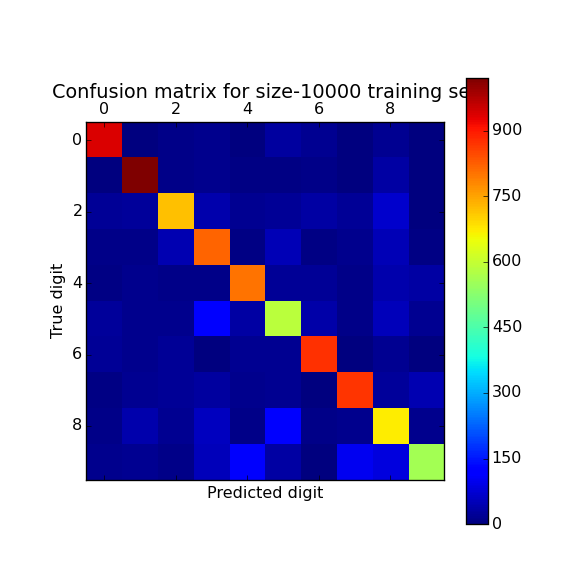
\includegraphics[scale=0.5]{images/confusion_matrix_10000} &
\end{tabular}
The algorithm seems to have fewer misclassifications as the training set size increases, but the added benefit at each increase also seems to decrease.


\newpage
\section*{Problem 3}
\stepcounter{problemnumber}
With $k$-fold cross validation, you can essentially use the entire given data set as training and validation. It also reduces the risk of overfitting because each of the $k$ folds takes a turn as the validation set while the classifier trains on the rest of the data. \asdf
The error rates seemed to hit a minimum of about $13.5\%$ around $C=2\cdot 10^{-7}$. Some data for accuracy-vs-C can be found in \texttt{digits\_out.txt}. Accuracy on the Kaggle test dataset was $87.64\%$.


\section*{Problem 4}
\stepcounter{problemnumber}
The optimal accuracy using cross validation was about $81.7\%$ using $C=92.86$. No features were added or removed. Some data for accuracy-vs-C can be found in \texttt{spam\_out.txt}. Accuracy on the Kaggle test dataset was $81.22\%$.

\end{document}
